\part{Study 2 Results}

\chapter{Overview of the registered outcome}
\label{r:ch:s2-overview}

All \RecStudyTwoRuns\ registered runs completed between \RecStudyTwoStart\ and \RecStudyTwoEnd~IST. None failed,
needed a retry, or diverged; every run was trained from the registration commit; every result matched its registered
split hash; and the collector reported no missing, duplicated, or mismatched task. The registered analysis
(\artifact{analysis/study2/run_all.sh}) ran once, on 19 October at 12:56.

\begin{longtable}{lp{0.42\textwidth}rrl}
\caption{The five registered Study 2 tests (H5 in pp of gap per pp of recoverability).}\label{r:tab:s2-verdicts}\\
\toprule
& Question & Estimate & Adjusted $p$ & Verdict \\
\midrule
\endfirsthead
\bottomrule
\endfoot
H1 & SIPaKMeD P1 $-$ P2 accuracy (primary, tested alone) & \HoneEst & \HoneP & \supported \\
H2 & CRIC P1 $-$ P2 accuracy & \HtwoEst & \HtwoPholm & \supported \\
H3 & Leakage at matched diversity (2C) & \HthreeEst & \HthreePholm & \supported \\
H4 & Own-context route through backgrounds (2B) & \HfourEst & \HfourPholm & \notsupported \\
H5 & Gap versus suppressed recoverability (2A) & \HfiveEst & \HfivePholm & \notsupported \\
\end{longtable}

Gate~A (H1 supported) means the inflation is reported as certified. Gate~B was ``murky'': H3 was supported but H4 was
not and H5 was not supported (one of two architectures failed its manipulation check). That is the result that motivated
Amendment~8.

\chapter{H1: crop-level splitting inflates SIPaKMeD accuracy}
\label{r:ch:h1}

\section{The registered test}

Mean test accuracy was \SipPOneAcc\% under P1 and \SipPTwoAcc\% under P2. The registered residual check flagged heavy
tails (residual skewness \RecHoneSkew, excess kurtosis \RecHoneKurt, Shapiro--Wilk $p$ \RecHoneShapiro), so, as registered,
the two-way cluster bootstrap is the primary inference: \HoneEst~pp (95\% interval \HoneBootLo--\HoneBootHi, bootstrap
$p$ \HoneBootP). Every sensitivity analysis agrees (Table~\ref{r:tab:sensitivity}): the mixed model gives the same
estimate with Satterthwaite $df=\HoneDf$ and $p$ \HoneKRp\ under Kenward--Roger, the seed-level sign-flip test gives $p$
\HoneSignFlipP, and the binomial mixed model a log odds ratio of \HoneGlmmLogOR\ ($p$ \HoneGlmmP).

\begin{figure}[H]
\centering
\begin{adjustbox}{max width=\textwidth}
\begin{tikzpicture}[node distance=5mm and 7mm]
\node[box=30mm] (fit) {Fit H1 model\\\footnotesize REML, bobyqa};
\node[gold=30mm, right=of fit] (conv) {Converged?\\\footnotesize singular accepted};
\node[box=30mm, right=of conv] (simp) {Simplify\\\footnotesize uncorrelated slope, then no seed intercept};
\node[gold=30mm, below=of conv] (assume) {Residual $|$skew$|>1$ or excess kurtosis $>3$?};
\node[done=30mm, left=of assume] (lmm) {Primary: Satterthwaite $t$-test};
\node[done=30mm, right=of assume] (boot) {Primary: two-way cluster bootstrap};
\node[box=95mm, below=6mm of assume] (sens) {Always reported: Kenward--Roger, binomial GLMM, seed sign-flip, bootstrap, per-architecture differences};
\draw[flow] (fit) -- (conv); \draw[flow] (conv) -- node[note, above]{no} (simp); \draw[flow] (simp.north) to[bend right=25] (fit.north);
\draw[flow] (conv) -- node[note, right]{yes} (assume); \draw[flow] (assume) -- node[note, above]{no} (lmm);
\draw[flow] (assume) -- node[note, above]{yes} (boot); \draw[flow] (assume) -- (sens);
\node[note, below=1mm of boot, text width=34mm] {Study 2: skew \RecHoneSkew, kurtosis \RecHoneKurt\ $\Rightarrow$ bootstrap};
\end{tikzpicture}
\end{adjustbox}
\caption{The registered H1 decision path. The residual check fired, so the cluster bootstrap became the primary inference
exactly as registered; every other method gave the same answer.}
\label{r:fig:h1-decision}
\end{figure}


\begin{figure}[H]
\centering
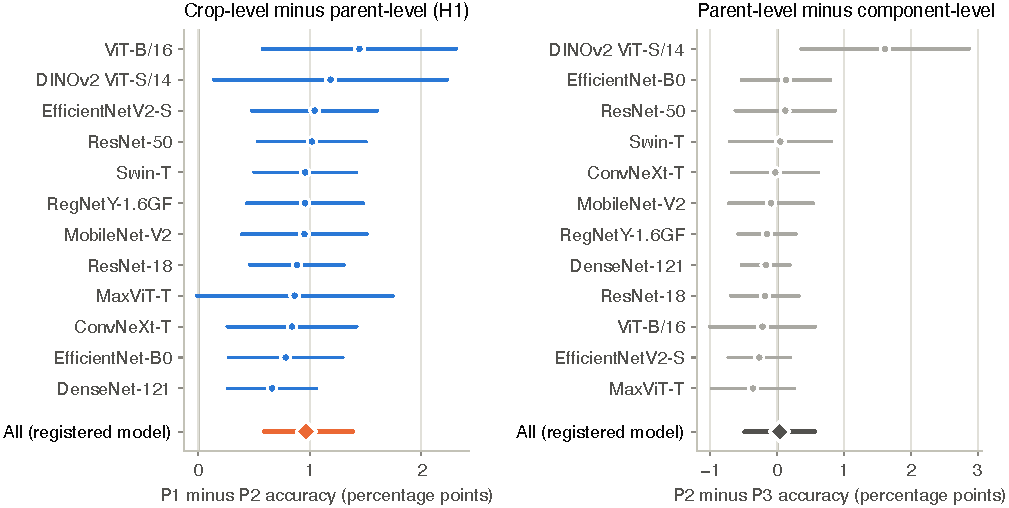
\includegraphics[width=\textwidth]{h1.pdf}
\caption{P1 $-$ P2 (left) and P2 $-$ P3 (right) per architecture (mean and 95\% $t$ interval over 20 seeds) with the
registered pooled estimates.}
\label{r:fig:h1}
\end{figure}

{\scriptsize
\setlength{\tabcolsep}{3.5pt}
\begin{longtable}{llrrrrrrrrl}
\caption{Every protocol model with its registered sensitivity analyses: Satterthwaite and Kenward--Roger degrees of freedom, two-way cluster bootstrap, and seed sign-flip test. The primary source is the bootstrap when the registered residual check fails.}\label{r:tab:sensitivity}\\
\toprule
Contrast & Model & Est. & SE & df$_S$ & $p_S$ & df$_{KR}$ & $p_{KR}$ & Bootstrap CI & Sign-flip $p$ & Primary \\
\midrule
\endfirsthead
\toprule
Contrast & Model & Est. & SE & df$_S$ & $p_S$ & df$_{KR}$ & $p_{KR}$ & Bootstrap CI & Sign-flip $p$ & Primary \\
\midrule
\endhead
\bottomrule
\endfoot
H1 accuracy & full & 0.97 & 0.17 & 38.8 & $<$0.001 & 18.8 & $<$0.001 & 0.59--1.39 & $<$0.001 & cluster\_bootstrap \\
H1 macro-F1 & full & 0.96 & 0.17 & 38.8 & $<$0.001 & 18.7 & $<$0.001 & 0.59--1.39 & $<$0.001 & cluster\_bootstrap \\
H1 balanced accuracy & full & 0.98 & 0.17 & 38.8 & $<$0.001 & 18.7 & $<$0.001 & 0.60--1.40 & $<$0.001 & cluster\_bootstrap \\
P2 $-$ P3 accuracy & full & 0.03 & 0.25 & 25.7 & 0.90 & 25.2 & 0.90 & \textminus{}0.45--0.60 & 0.88 & lmm \\
H2 CRIC accuracy & full & 12.08 & 0.40 & 8.8 & $<$0.001 & 8.8 & $<$0.001 & 11.23--12.92 & 0.002 & lmm \\
CRIC P1$'$ $-$ P2 & full & 12.11 & 0.43 & 17.5 & $<$0.001 & 10.1 & $<$0.001 & 11.21--13.05 & 0.002 & lmm \\
CRIC balanced accuracy & full & 19.64 & 0.71 & 18.0 & $<$0.001 & 7.2 & $<$0.001 & 18.00--21.34 & 0.002 & lmm \\
CRIC macro-F1 & full & 20.59 & 0.60 & 6.3 & $<$0.001 & 6.3 & $<$0.001 & 19.19--22.02 & 0.002 & lmm \\
\end{longtable}
}


\section{Consistency}

All \HonePositiveArchs\ architectures scored higher under P1 (\HoneArchMin--\HoneArchMax~pp) and \HoneArchCIPositive\ of
them individually had intervals excluding zero. At the seed level the picture is noisier but one-sided
(Figure~\ref{r:fig:seed-heatmap}). The parent-level error rate is \SipErrorRatio\ times the crop-level one. Macro-F1
(\HoneFoneEst~pp) and balanced accuracy (\HoneBaccEst~pp) moved by the same amount.

\begin{figure}[H]
\centering
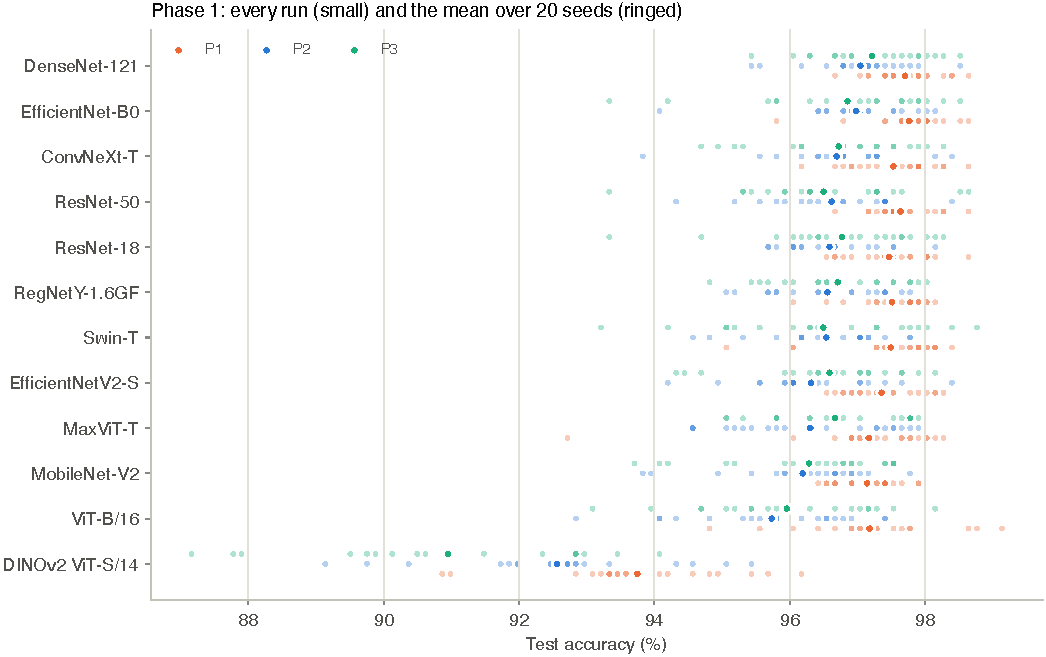
\includegraphics[width=\textwidth]{phase1_points.pdf}
\caption{Every Phase~1 run and the per-protocol mean over 20 seeds, by architecture.}
\label{r:fig:phase1-points}
\end{figure}

\begin{figure}[H]
\centering
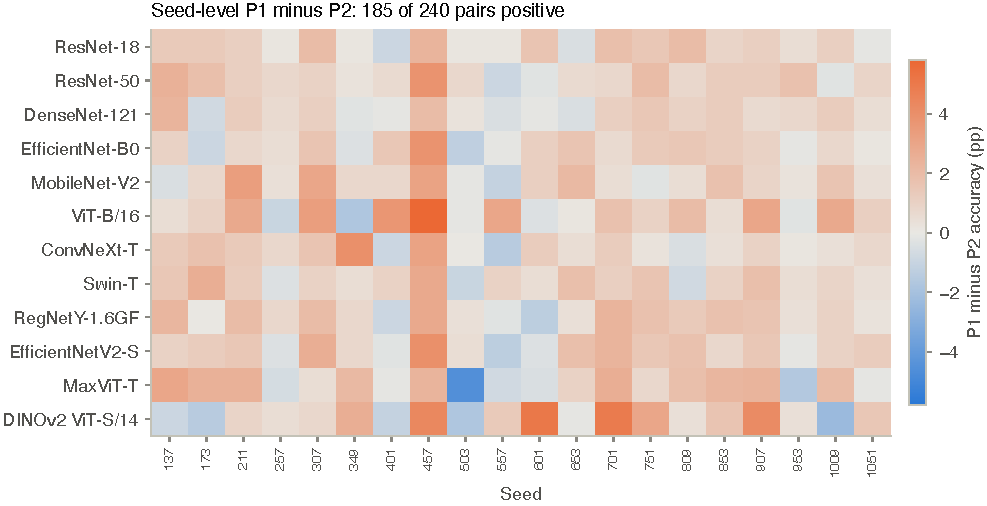
\includegraphics[width=\textwidth]{seed_heatmap.pdf}
\caption{P1 $-$ P2 accuracy for every architecture and seed (diverging scale, zero in grey).}
\label{r:fig:seed-heatmap}
\end{figure}

\begin{figure}[H]
\centering
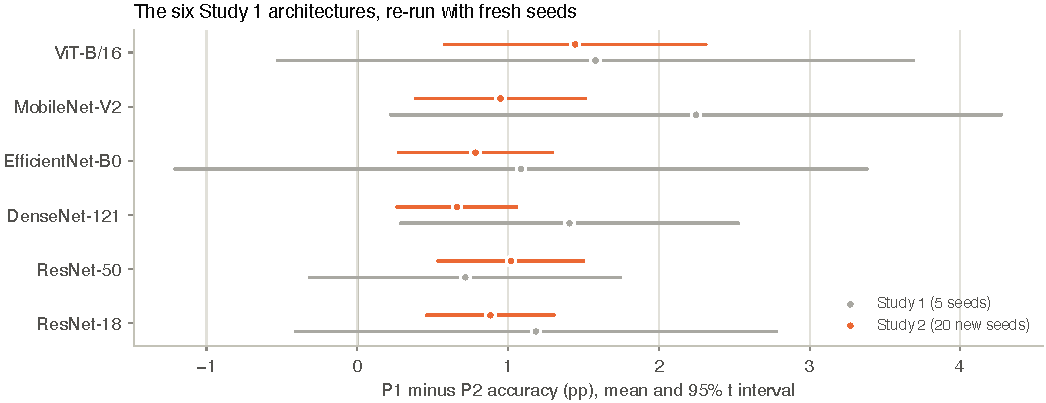
\includegraphics[width=\textwidth]{cross_study.pdf}
\caption{The six Study~1 architectures: Study~1's five-seed estimates and Study~2's twenty-seed estimates of P1 $-$ P2.
Study~2's intervals are narrower and all exclude zero.}
\label{r:fig:cross-study}
\end{figure}

\section{P2 versus P3, rankings, and the ordering gate}

Merging near-duplicate-linked parents on top of parent-level splitting changed nothing (P2 $-$ P3 \PtwoPthreeEst~pp,
\PtwoPthreeLo\ to \PtwoPthreeHi, $p=\PtwoPthreeP$). The registered P3 $\leq$ P2 $\leq$ P1 ordering passed for
\RecOrderingPassed\ of twelve architectures, as expected when two protocols are equivalent and the order between them is
decided by noise. The architecture ranking was largely preserved between P1 and P2 (Kendall $\tau=\KendallTau$,
\KendallLo--\KendallHi; \ReorderedPairs\ pairs reordered).

\section{Crop-level evidence}

Within crops that were test crops under both protocols in different seeds (\MoneCrops\ crops), accuracy was \MoneEst~pp
higher under P1 (\MoneLo--\MoneHi; M1). Within P1, a crop sharing source pixels with a training crop was more often
correct (log odds \MtwoOverlapLogOdds, $p$ \MtwoOverlapP), as was a crop with more training siblings (log odds
\MtwoSiblingsLogOdds\ per log sibling, $p=\MtwoSiblingsP$), adjusting for class and the crop's difficulty under P2 (M2).

\section{Training behaviour}

\begin{figure}[H]
\centering
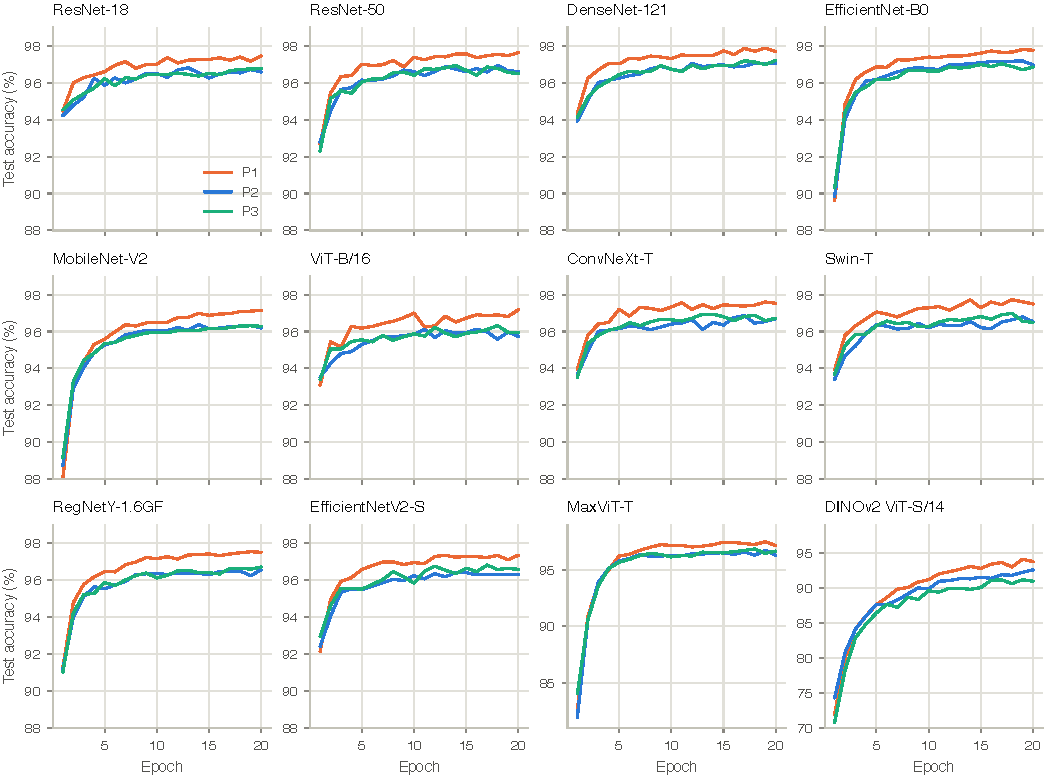
\includegraphics[width=\textwidth]{training_curves.pdf}
\caption{Mean test accuracy per epoch under P1, P2, and P3 (20 seeds each). The P1 advantage appears within the first
few epochs and persists to the final-epoch endpoint.}
\label{r:fig:training-curves}
\end{figure}

\begin{figure}[H]
\centering
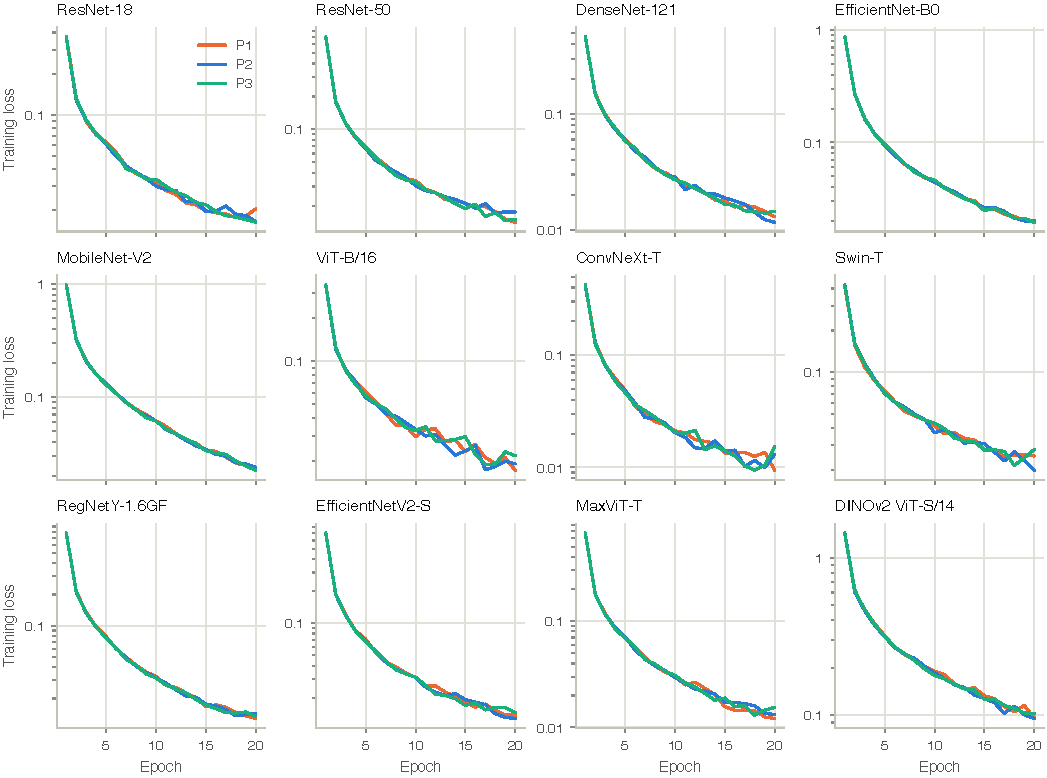
\includegraphics[width=\textwidth]{loss_curves.pdf}
\caption{Mean training loss per epoch (log scale). Training is indistinguishable across protocols; the difference is in
what the test set contains, not in how training proceeds.}
\label{r:fig:loss-curves}
\end{figure}

\section{Calibration and errors}

Pooled over runs, the 15-bin expected calibration error was \RecEceOne\% under P1, \RecEceTwo\% under P2, and
\RecEceThree\% under P3, and the negative log-likelihood \RecNllOne, \RecNllTwo, and \RecNllThree\ nats: crop-level
splits flatter calibration as well as accuracy.

\begin{figure}[H]
\centering
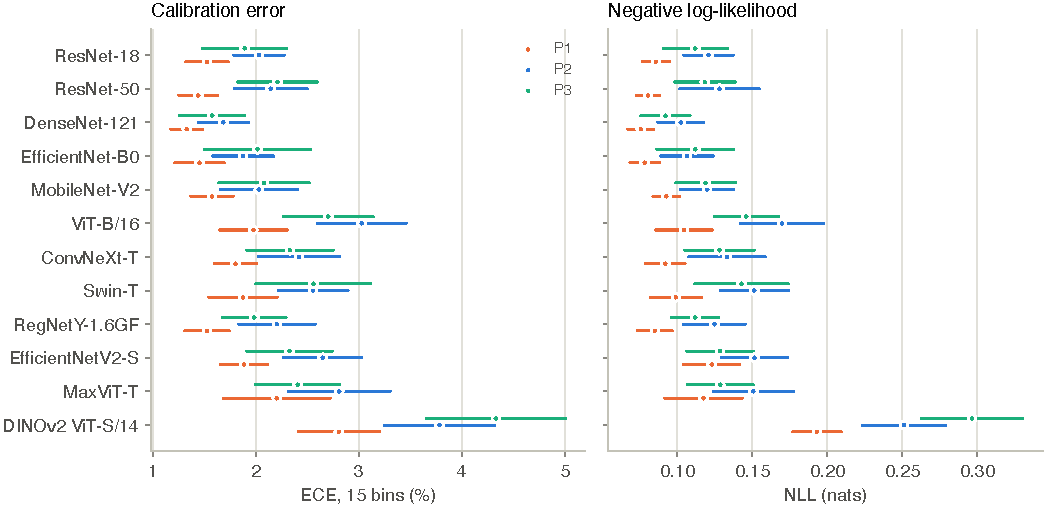
\includegraphics[width=\textwidth]{calibration.pdf}
\caption{Calibration error and negative log-likelihood by architecture and protocol (mean and 95\% $t$ interval).}
\label{r:fig:calibration}
\end{figure}

{\footnotesize
\setlength{\tabcolsep}{3.5pt}
\begin{longtable}{llrrrrr}
\caption{Phase 1 (SIPaKMeD, 20 seeds per cell): test metrics in percent (mean\,$\pm$\,SD over seeds); NLL in nats.}\label{r:tab:phase1}\\
\toprule
Architecture & Prot. & Accuracy & Macro-F1 & Balanced acc. & ECE & NLL \\
\midrule
\endfirsthead
\toprule
Architecture & Prot. & Accuracy & Macro-F1 & Balanced acc. & ECE & NLL \\
\midrule
\endhead
\bottomrule
\endfoot
ResNet-18 & P1 & 97.47\,$\pm$\,0.56 & 97.48\,$\pm$\,0.56 & 97.49\,$\pm$\,0.56 & 1.52\,$\pm$\,0.44 & 0.086 \\
 & P2 & 96.59\,$\pm$\,0.68 & 96.60\,$\pm$\,0.67 & 96.59\,$\pm$\,0.68 & 2.03\,$\pm$\,0.53 & 0.121 \\
 & P3 & 96.77\,$\pm$\,1.22 & 96.78\,$\pm$\,1.21 & 96.77\,$\pm$\,1.21 & 1.89\,$\pm$\,0.87 & 0.112 \\
ResNet-50 & P1 & 97.64\,$\pm$\,0.46 & 97.65\,$\pm$\,0.45 & 97.65\,$\pm$\,0.46 & 1.44\,$\pm$\,0.40 & 0.080 \\
 & P2 & 96.62\,$\pm$\,0.94 & 96.63\,$\pm$\,0.94 & 96.62\,$\pm$\,0.94 & 2.14\,$\pm$\,0.75 & 0.128 \\
 & P3 & 96.50\,$\pm$\,1.23 & 96.51\,$\pm$\,1.23 & 96.49\,$\pm$\,1.26 & 2.21\,$\pm$\,0.82 & 0.118 \\
DenseNet-121 & P1 & 97.70\,$\pm$\,0.51 & 97.71\,$\pm$\,0.51 & 97.72\,$\pm$\,0.51 & 1.33\,$\pm$\,0.33 & 0.076 \\
 & P2 & 97.04\,$\pm$\,0.74 & 97.05\,$\pm$\,0.74 & 97.05\,$\pm$\,0.74 & 1.68\,$\pm$\,0.52 & 0.102 \\
 & P3 & 97.22\,$\pm$\,0.83 & 97.23\,$\pm$\,0.83 & 97.21\,$\pm$\,0.83 & 1.57\,$\pm$\,0.68 & 0.092 \\
EfficientNet-B0 & P1 & 97.77\,$\pm$\,0.61 & 97.77\,$\pm$\,0.62 & 97.78\,$\pm$\,0.61 & 1.45\,$\pm$\,0.51 & 0.078 \\
 & P2 & 96.98\,$\pm$\,0.86 & 96.98\,$\pm$\,0.87 & 96.99\,$\pm$\,0.85 & 1.87\,$\pm$\,0.64 & 0.106 \\
 & P3 & 96.85\,$\pm$\,1.35 & 96.86\,$\pm$\,1.34 & 96.86\,$\pm$\,1.34 & 2.01\,$\pm$\,1.10 & 0.112 \\
MobileNet-V2 & P1 & 97.14\,$\pm$\,0.46 & 97.15\,$\pm$\,0.46 & 97.16\,$\pm$\,0.46 & 1.57\,$\pm$\,0.44 & 0.093 \\
 & P2 & 96.19\,$\pm$\,1.01 & 96.20\,$\pm$\,1.01 & 96.19\,$\pm$\,1.02 & 2.03\,$\pm$\,0.80 & 0.120 \\
 & P3 & 96.28\,$\pm$\,1.22 & 96.29\,$\pm$\,1.22 & 96.28\,$\pm$\,1.22 & 2.08\,$\pm$\,0.94 & 0.119 \\
ViT-B/16 & P1 & 97.18\,$\pm$\,1.03 & 97.19\,$\pm$\,1.02 & 97.19\,$\pm$\,1.04 & 1.97\,$\pm$\,0.70 & 0.104 \\
 & P2 & 95.73\,$\pm$\,1.21 & 95.73\,$\pm$\,1.23 & 95.74\,$\pm$\,1.21 & 3.02\,$\pm$\,0.92 & 0.170 \\
 & P3 & 95.96\,$\pm$\,1.30 & 95.96\,$\pm$\,1.31 & 95.97\,$\pm$\,1.30 & 2.70\,$\pm$\,0.93 & 0.146 \\
ConvNeXt-T & P1 & 97.53\,$\pm$\,0.64 & 97.54\,$\pm$\,0.63 & 97.54\,$\pm$\,0.64 & 1.80\,$\pm$\,0.43 & 0.092 \\
 & P2 & 96.69\,$\pm$\,0.95 & 96.70\,$\pm$\,0.94 & 96.69\,$\pm$\,0.95 & 2.42\,$\pm$\,0.84 & 0.133 \\
 & P3 & 96.72\,$\pm$\,1.06 & 96.72\,$\pm$\,1.07 & 96.73\,$\pm$\,1.05 & 2.33\,$\pm$\,0.89 & 0.128 \\
Swin-T & P1 & 97.49\,$\pm$\,0.84 & 97.50\,$\pm$\,0.84 & 97.51\,$\pm$\,0.84 & 1.87\,$\pm$\,0.71 & 0.099 \\
 & P2 & 96.54\,$\pm$\,0.89 & 96.55\,$\pm$\,0.88 & 96.55\,$\pm$\,0.88 & 2.55\,$\pm$\,0.72 & 0.151 \\
 & P3 & 96.49\,$\pm$\,1.46 & 96.50\,$\pm$\,1.47 & 96.50\,$\pm$\,1.46 & 2.56\,$\pm$\,1.19 & 0.143 \\
RegNetY-1.6GF & P1 & 97.51\,$\pm$\,0.54 & 97.52\,$\pm$\,0.54 & 97.53\,$\pm$\,0.54 & 1.52\,$\pm$\,0.47 & 0.085 \\
 & P2 & 96.56\,$\pm$\,0.83 & 96.57\,$\pm$\,0.84 & 96.56\,$\pm$\,0.83 & 2.20\,$\pm$\,0.79 & 0.125 \\
 & P3 & 96.71\,$\pm$\,0.93 & 96.72\,$\pm$\,0.94 & 96.71\,$\pm$\,0.93 & 1.98\,$\pm$\,0.66 & 0.112 \\
EfficientNetV2-S & P1 & 97.36\,$\pm$\,0.54 & 97.37\,$\pm$\,0.54 & 97.37\,$\pm$\,0.53 & 1.88\,$\pm$\,0.49 & 0.123 \\
 & P2 & 96.31\,$\pm$\,0.95 & 96.32\,$\pm$\,0.96 & 96.32\,$\pm$\,0.95 & 2.65\,$\pm$\,0.81 & 0.151 \\
 & P3 & 96.59\,$\pm$\,1.09 & 96.59\,$\pm$\,1.09 & 96.59\,$\pm$\,1.09 & 2.32\,$\pm$\,0.88 & 0.128 \\
MaxViT-T & P1 & 97.17\,$\pm$\,1.19 & 97.17\,$\pm$\,1.20 & 97.19\,$\pm$\,1.18 & 2.20\,$\pm$\,1.11 & 0.117 \\
 & P2 & 96.30\,$\pm$\,1.21 & 96.31\,$\pm$\,1.20 & 96.31\,$\pm$\,1.21 & 2.81\,$\pm$\,1.06 & 0.151 \\
 & P3 & 96.67\,$\pm$\,0.97 & 96.67\,$\pm$\,0.98 & 96.68\,$\pm$\,0.97 & 2.40\,$\pm$\,0.87 & 0.129 \\
DINOv2 ViT-S/14 & P1 & 93.75\,$\pm$\,1.34 & 93.78\,$\pm$\,1.33 & 93.79\,$\pm$\,1.33 & 2.80\,$\pm$\,0.85 & 0.193 \\
 & P2 & 92.56\,$\pm$\,1.60 & 92.61\,$\pm$\,1.55 & 92.61\,$\pm$\,1.60 & 3.78\,$\pm$\,1.15 & 0.251 \\
 & P3 & 90.95\,$\pm$\,1.95 & 90.99\,$\pm$\,1.92 & 90.99\,$\pm$\,1.95 & 4.33\,$\pm$\,1.45 & 0.297 \\
\end{longtable}
}


\chapter{H2: the CRIC inflation is an order of magnitude larger}
\label{r:ch:h2}

CRIC accuracy fell from \CricPOneAcc\% under crop-level splitting to \CricPTwoAcc\% under slide-level splitting:
H2 $=$ \HtwoEst~pp (\HtwoLo--\HtwoHi; Holm $p$ \HtwoPholm). The error rate rose \CricErrorRatio-fold. Because the classes
are imbalanced, balanced accuracy fell further, from \CricPOneBacc\% to \CricPTwoBacc\% (\CricBaccEst~pp), and macro-F1 by
\CricFoneEst~pp. The size-matched P1-prime gave the same inflation (\CricPrimeEst~pp), so it is not a training-size
effect.

\begin{figure}[H]
\centering
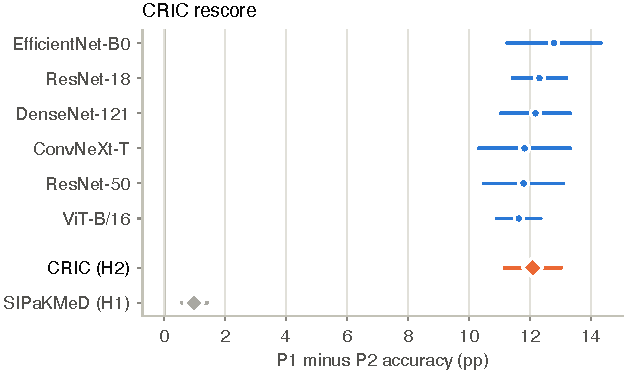
\includegraphics[width=0.85\textwidth]{cric.pdf}
\caption{CRIC P1 $-$ P2 per architecture, the registered estimate, and the SIPaKMeD estimate for scale.}
\label{r:fig:cric}
\end{figure}

The loss is concentrated in the abnormal classes (Figure~\ref{r:fig:cric-recall}). Recall for ASC-H, LSIL, and HSIL falls
by tens of points when slides are held out, while the majority NILM class barely moves; the crop-level split had been
rewarding the recognition of slides whose abnormal cells were already seen.

\begin{figure}[H]
\centering
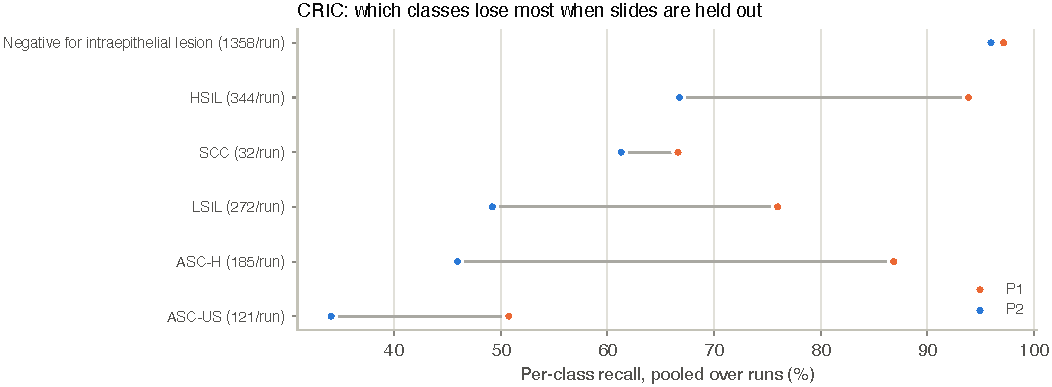
\includegraphics[width=\textwidth]{cric_recall.pdf}
\caption{CRIC per-class recall under P1 and P2, pooled over all runs, with the mean number of test cells per class.}
\label{r:fig:cric-recall}
\end{figure}

\begin{figure}[H]
\centering
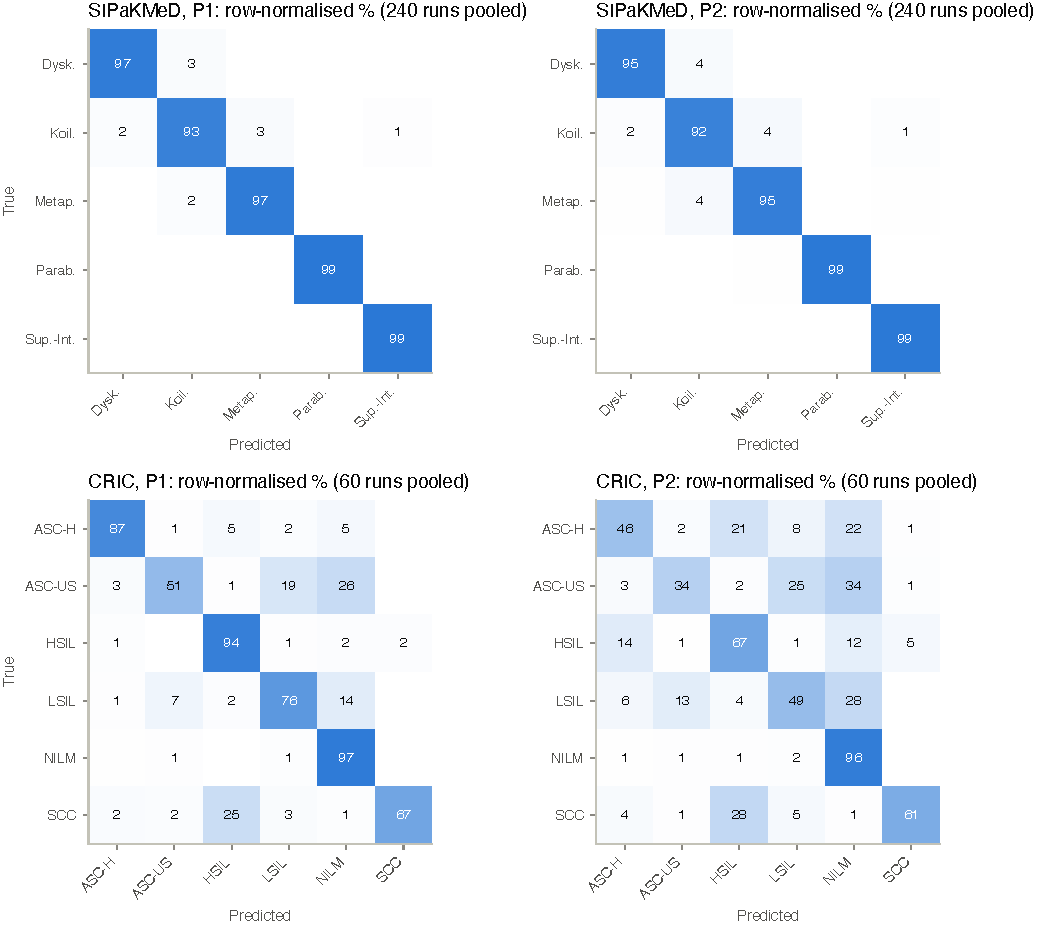
\includegraphics[width=\textwidth]{confusion.pdf}
\caption{Row-normalised confusion matrices pooled over runs. SIPaKMeD errors barely change between protocols; CRIC's
abnormal classes collapse toward NILM and toward each other under slide-level splitting.}
\label{r:fig:confusion}
\end{figure}

{\footnotesize
\setlength{\tabcolsep}{3.5pt}
\begin{longtable}{llrrrrr}
\caption{CRIC (10 seeds per cell): test metrics in percent (mean\,$\pm$\,SD).}\label{r:tab:cric}\\
\toprule
Architecture & Prot. & Accuracy & Macro-F1 & Balanced acc. & ECE & NLL \\
\midrule
\endfirsthead
\toprule
Architecture & Prot. & Accuracy & Macro-F1 & Balanced acc. & ECE & NLL \\
\midrule
\endhead
\bottomrule
\endfoot
ResNet-18 & P1 & 89.91\,$\pm$\,0.43 & 79.09\,$\pm$\,1.31 & 77.60\,$\pm$\,2.07 & 5.50\,$\pm$\,0.40 & 0.383 \\
 & P1-prime & 89.92\,$\pm$\,0.68 & 78.94\,$\pm$\,1.43 & 77.42\,$\pm$\,2.25 & 5.48\,$\pm$\,0.67 & 0.387 \\
 & P2 & 77.62\,$\pm$\,1.14 & 57.25\,$\pm$\,1.45 & 56.79\,$\pm$\,2.63 & 14.98\,$\pm$\,1.11 & 1.014 \\
ResNet-50 & P1 & 90.54\,$\pm$\,0.48 & 80.48\,$\pm$\,1.63 & 79.42\,$\pm$\,2.41 & 5.85\,$\pm$\,0.33 & 0.388 \\
 & P1-prime & 90.85\,$\pm$\,0.62 & 81.01\,$\pm$\,1.66 & 79.85\,$\pm$\,2.02 & 5.41\,$\pm$\,0.45 & 0.371 \\
 & P2 & 78.76\,$\pm$\,1.80 & 60.48\,$\pm$\,3.30 & 60.34\,$\pm$\,2.84 & 14.97\,$\pm$\,1.82 & 0.995 \\
DenseNet-121 & P1 & 90.40\,$\pm$\,0.74 & 79.66\,$\pm$\,1.93 & 77.97\,$\pm$\,2.71 & 5.42\,$\pm$\,0.68 & 0.374 \\
 & P1-prime & 90.71\,$\pm$\,0.48 & 80.22\,$\pm$\,1.41 & 78.32\,$\pm$\,1.76 & 5.36\,$\pm$\,0.46 & 0.365 \\
 & P2 & 78.23\,$\pm$\,1.50 & 59.08\,$\pm$\,2.36 & 58.82\,$\pm$\,2.77 & 14.95\,$\pm$\,1.28 & 1.017 \\
EfficientNet-B0 & P1 & 90.88\,$\pm$\,0.53 & 80.74\,$\pm$\,0.99 & 79.78\,$\pm$\,1.46 & 5.33\,$\pm$\,0.43 & 0.370 \\
 & P1-prime & 90.95\,$\pm$\,0.60 & 80.95\,$\pm$\,1.05 & 80.83\,$\pm$\,1.64 & 5.21\,$\pm$\,0.54 & 0.363 \\
 & P2 & 78.10\,$\pm$\,2.15 & 58.73\,$\pm$\,2.78 & 59.86\,$\pm$\,2.19 & 14.90\,$\pm$\,1.74 & 1.021 \\
ViT-B/16 & P1 & 89.83\,$\pm$\,0.63 & 78.01\,$\pm$\,2.30 & 76.37\,$\pm$\,3.22 & 6.54\,$\pm$\,0.95 & 0.436 \\
 & P1-prime & 89.54\,$\pm$\,0.70 & 78.28\,$\pm$\,1.81 & 76.45\,$\pm$\,2.95 & 6.55\,$\pm$\,0.68 & 0.429 \\
 & P2 & 78.20\,$\pm$\,1.13 & 59.54\,$\pm$\,1.47 & 57.62\,$\pm$\,2.28 & 16.14\,$\pm$\,1.29 & 1.054 \\
ConvNeXt-T & P1 & 91.29\,$\pm$\,0.63 & 81.80\,$\pm$\,1.57 & 80.03\,$\pm$\,2.69 & 5.91\,$\pm$\,0.58 & 0.392 \\
 & P1-prime & 91.10\,$\pm$\,0.40 & 80.73\,$\pm$\,1.97 & 78.85\,$\pm$\,2.17 & 6.02\,$\pm$\,0.53 & 0.392 \\
 & P2 & 79.48\,$\pm$\,1.78 & 61.15\,$\pm$\,3.27 & 59.90\,$\pm$\,3.99 & 15.82\,$\pm$\,1.76 & 1.082 \\
\end{longtable}
}


\chapter{H3: the inflation is leakage, not training diversity}
\label{r:ch:h3}

With crop count, field count, and allocation rule held equal, adding the test fields' sibling crops to training raised
accuracy on the common test set by \HthreeEst~pp (\HthreeLo--\HthreeHi; Holm $p=\HthreePholm$). Every architecture showed
it at both diversity levels (Figure~\ref{r:fig:factorial-cells}). Increasing the number of distinct training fields from
504 to 720 without leakage did nothing (\DivEst~pp, \DivLo\ to \DivHi), and the leak effect did not depend on diversity
(interaction \InteractionEst~pp, $p=\InteractionP$). The registered approximate decomposition assigns the Phase~1 gap
entirely to leakage (diversity component \DecompDiv~pp).

\begin{figure}[H]
\centering
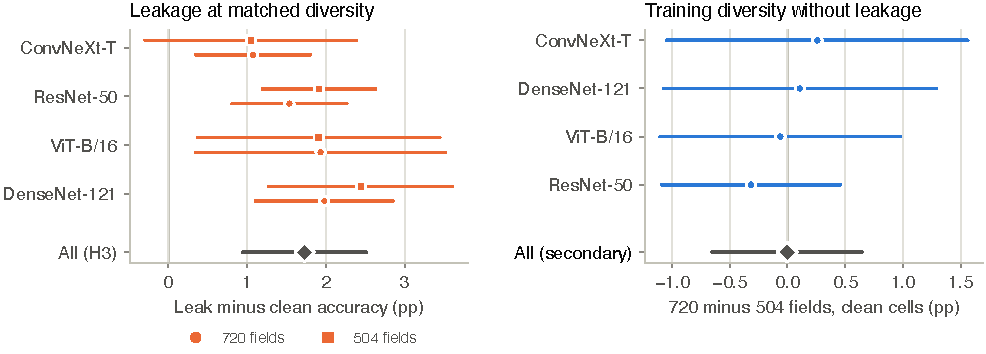
\includegraphics[width=\textwidth]{factorial.pdf}
\caption{Left: leak minus clean accuracy per architecture and diversity level, and the H3 estimate. Right: high minus
low diversity within clean cells.}
\label{r:fig:factorial}
\end{figure}

\begin{figure}[H]
\centering
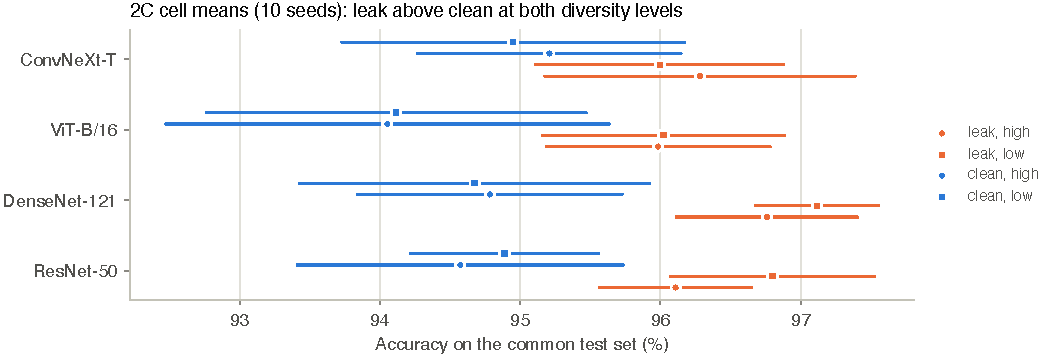
\includegraphics[width=\textwidth]{factorial_cells.pdf}
\caption{All four 2C cell means per architecture (10 seeds each).}
\label{r:fig:factorial-cells}
\end{figure}

The diversity manipulation did change what the training sets contain. In the embedding space of a retrained parent-probe
encoder (which identified held-out fields at \RecEncoderAcc\% against \RecEncoderChance\% chance), the mean distance between
field centroids was \RecDivCleanHigh\ for 720-field and \RecDivCleanLow\ for 504-field clean training sets, and
\RecDivPOne\ (P1, \RecDivParentsPOne\ fields) against \RecDivPTwo\ (P2, \RecDivParentsPTwo\ fields) for the natural splits.
More diverse training sets were measurably more diverse; that diversity simply did not improve accuracy.

\chapter{H4: background transplants do not isolate the route}
\label{r:ch:h4}

\begin{figure}[H]
\centering
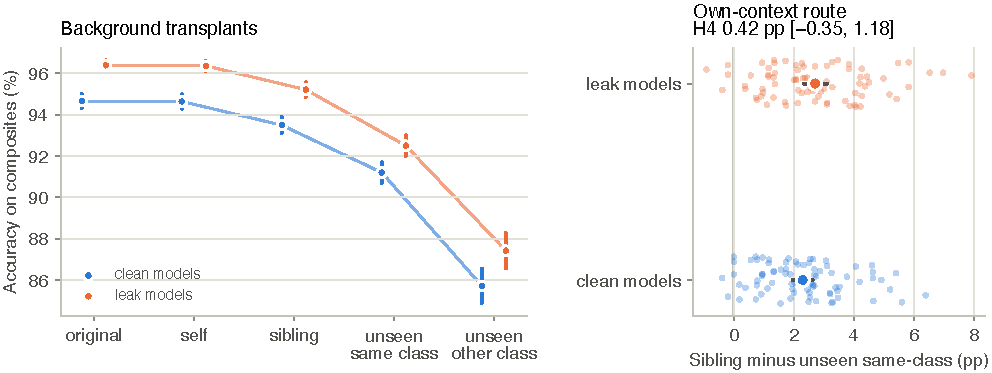
\includegraphics[width=\textwidth]{transplant.pdf}
\caption{Left: accuracy of leak and clean models on composites of the common test set. Right: the per-run own-context
route and the registered H4 contrast.}
\label{r:fig:transplant}
\end{figure}

Compositing a cell onto its own inpainted background cost nothing, so seam and inpainting artifacts were negligible.
Leak models were \LeakOriginalEst~pp more accurate than clean models on unmodified cells and kept most of that advantage
when the background was replaced: \TransplantLeakSibling~pp on sibling backgrounds, \TransplantLeakUnseen~pp on backgrounds
from unseen fields of the same class, and \TransplantLeakOther~pp on other-class backgrounds. H4, the leak-minus-clean
difference of the own-context route, was \HfourEst~pp (\HfourLo\ to \HfourHi; Holm $p=\HfourPholm$): not supported. Its
point estimate would assign \RouteShare\% of the inflation to the background.

Two observations qualify the design. Sibling backgrounds helped even clean models, which had never seen those fields, by
\TransplantCleanHarmony~pp, presumably because a background from the cell's own field matches its stain; that effect is
common to both arms but inflates the variance of the contrast. And backgrounds do carry class information: an other-class
background moved \DonorShiftEst~pp of probability toward its class (\DonorShiftLo--\DonorShiftHi, secondary). Restricting H4
to recipients whose background covers at least 30\% of the crop gave \HfourBgEst~pp (\HfourBgLo\ to \HfourBgHi).

\begin{figure}[H]
\centering
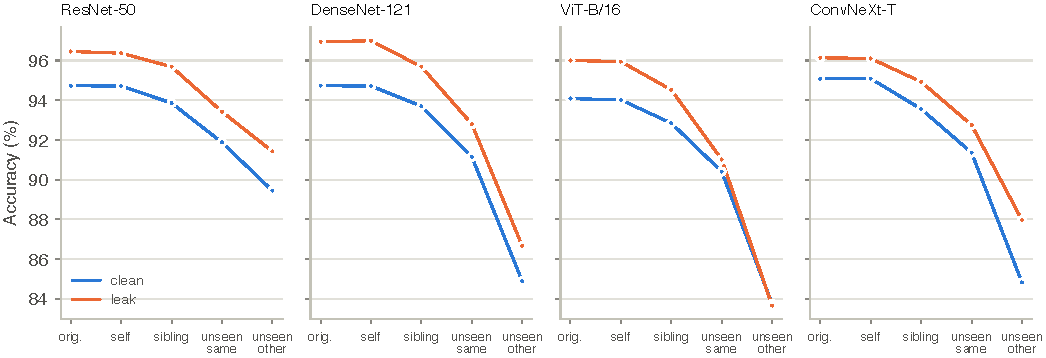
\includegraphics[width=\textwidth]{transplant_arch.pdf}
\caption{Transplant-condition accuracy of leak and clean models per architecture.}
\label{r:fig:transplant-arch}
\end{figure}

{\scriptsize
\setlength{\tabcolsep}{3.5pt}
\begin{longtable}{llrrrrrr}
\caption{2C/2B (10 seeds per cell): accuracy on the common test set and on each background-transplant condition (percent), and the donor-class probability shift (pp).}\label{r:tab:factorial}\\
\toprule
Architecture & Cell & Original & Self & Sibling & Unseen same & Unseen other & Shift \\
\midrule
\endfirsthead
\toprule
Architecture & Cell & Original & Self & Sibling & Unseen same & Unseen other & Shift \\
\midrule
\endhead
\bottomrule
\endfoot
ResNet-50 & leak\_high & 96.11\,$\pm$\,0.76 & 95.96\,$\pm$\,0.77 & 95.29\,$\pm$\,0.89 & 92.61\,$\pm$\,1.41 & 90.89\,$\pm$\,1.24 & 1.19 \\
 & clean\_high & 94.57\,$\pm$\,1.63 & 94.50\,$\pm$\,1.78 & 93.43\,$\pm$\,2.06 & 91.73\,$\pm$\,1.94 & 89.03\,$\pm$\,2.49 & 1.35 \\
 & leak\_low & 96.80\,$\pm$\,1.02 & 96.78\,$\pm$\,1.03 & 96.08\,$\pm$\,1.03 & 94.23\,$\pm$\,1.40 & 91.95\,$\pm$\,1.50 & 1.33 \\
 & clean\_low & 94.89\,$\pm$\,0.94 & 94.93\,$\pm$\,0.83 & 94.28\,$\pm$\,0.84 & 92.02\,$\pm$\,1.20 & 89.85\,$\pm$\,1.16 & 1.22 \\
DenseNet-121 & leak\_high & 96.76\,$\pm$\,0.91 & 96.89\,$\pm$\,0.77 & 95.67\,$\pm$\,0.60 & 92.80\,$\pm$\,1.51 & 86.79\,$\pm$\,1.96 & 4.15 \\
 & clean\_high & 94.78\,$\pm$\,1.32 & 94.78\,$\pm$\,1.26 & 93.72\,$\pm$\,1.20 & 90.97\,$\pm$\,1.99 & 84.58\,$\pm$\,2.57 & 4.50 \\
 & leak\_low & 97.12\,$\pm$\,0.62 & 97.10\,$\pm$\,0.65 & 95.70\,$\pm$\,1.28 & 92.80\,$\pm$\,2.21 & 86.52\,$\pm$\,2.90 & 4.36 \\
 & clean\_low & 94.67\,$\pm$\,1.75 & 94.65\,$\pm$\,1.83 & 93.68\,$\pm$\,1.63 & 91.33\,$\pm$\,2.28 & 85.19\,$\pm$\,3.46 & 4.08 \\
ViT-B/16 & leak\_high & 95.98\,$\pm$\,1.12 & 95.93\,$\pm$\,1.22 & 94.55\,$\pm$\,2.45 & 90.44\,$\pm$\,2.89 & 84.05\,$\pm$\,3.05 & 3.66 \\
 & clean\_high & 94.05\,$\pm$\,2.21 & 94.05\,$\pm$\,2.18 & 92.82\,$\pm$\,2.27 & 90.73\,$\pm$\,2.43 & 84.62\,$\pm$\,4.51 & 3.36 \\
 & leak\_low & 96.02\,$\pm$\,1.21 & 95.96\,$\pm$\,1.25 & 94.49\,$\pm$\,1.36 & 91.58\,$\pm$\,2.25 & 83.26\,$\pm$\,3.68 & 4.39 \\
 & clean\_low & 94.11\,$\pm$\,1.90 & 93.98\,$\pm$\,1.97 & 92.86\,$\pm$\,2.61 & 90.07\,$\pm$\,3.20 & 82.87\,$\pm$\,3.39 & 3.93 \\
ConvNeXt-T & leak\_high & 96.28\,$\pm$\,1.55 & 96.25\,$\pm$\,1.63 & 95.01\,$\pm$\,1.34 & 92.69\,$\pm$\,1.81 & 87.79\,$\pm$\,3.44 & 2.71 \\
 & clean\_high & 95.21\,$\pm$\,1.31 & 95.19\,$\pm$\,1.22 & 93.89\,$\pm$\,1.32 & 91.83\,$\pm$\,2.40 & 85.63\,$\pm$\,2.63 & 3.03 \\
 & leak\_low & 96.00\,$\pm$\,1.24 & 95.96\,$\pm$\,1.17 & 94.84\,$\pm$\,2.61 & 92.81\,$\pm$\,3.30 & 88.13\,$\pm$\,3.33 & 2.81 \\
 & clean\_low & 94.95\,$\pm$\,1.71 & 94.99\,$\pm$\,1.66 & 93.22\,$\pm$\,2.09 & 90.89\,$\pm$\,2.82 & 84.00\,$\pm$\,4.02 & 3.40 \\
\end{longtable}
}


\chapter{H5: gradient reversal was evaded}
\label{r:ch:h5}

\begin{figure}[H]
\centering
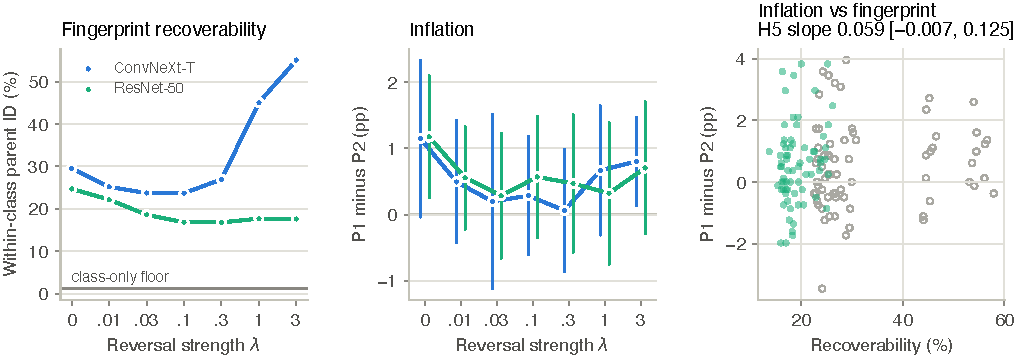
\includegraphics[width=\textwidth]{grl.pdf}
\caption{The gradient-reversal sweep: probe recoverability, the P1 $-$ P2 gap, and their relation (ConvNeXt-T, which
failed its manipulation check, hollow).}
\label{r:fig:grl}
\end{figure}

For ConvNeXt-T the adversary was evaded: as the reversal strength grew, an independent linear probe identified the field
\emph{better} (\GrlConvRzero\% at $\lambda=0$, \GrlConvRstar\% at $\lambda=3$), while the adversary's own training accuracy
fell toward chance (Figure~\ref{r:fig:grl-full}). The encoder learned features its two-layer adversary could not read but a
standardised linear probe could, the failure mode described for adversarial removal in language
models~\citep{elazar2018adversarial}. ConvNeXt-T therefore failed the registered manipulation check and was excluded. For
ResNet-50, recoverability fell from \GrlResRzero\% to \GrlResRstar\% and the mean gap fell from \GrlResGapZero~pp to
between \GrlResGapMin\ and \GrlResGapMax~pp at every $\lambda>0$, with P2 accuracy within 1~pp. The registered slope was
positive but not significant (\HfiveEst\ pp per pp, \HfiveLo\ to \HfiveHi; Holm $p=\HfivePholm$). Amendment~8's linear
adversary later showed the ResNet-50 gap does not fall when recoverability is suppressed on fresh seeds (Part~VI), so this
drop was most likely noise.

\begin{figure}[H]
\centering
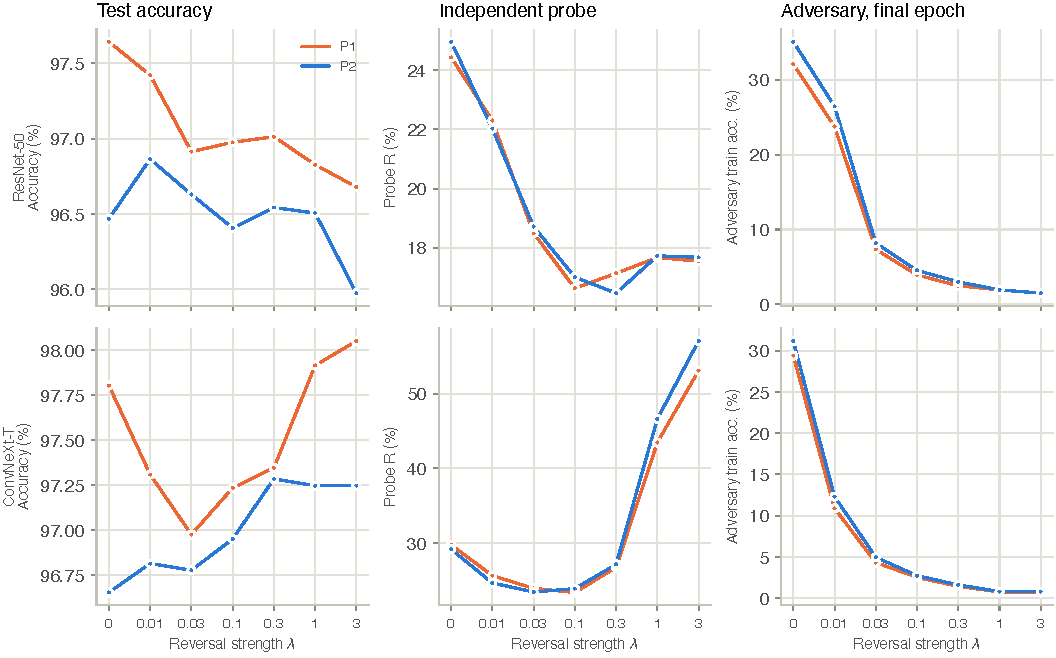
\includegraphics[width=\textwidth]{grl_full.pdf}
\caption{The full 2A sweep per architecture: test accuracy, independent-probe recoverability, and the adversary's own
within-class training accuracy at the final epoch.}
\label{r:fig:grl-full}
\end{figure}

{\footnotesize
\setlength{\tabcolsep}{3.5pt}
\begin{longtable}{lrrrrrr}
\caption{2A gradient-reversal sweep (10 seeds): accuracy (percent), mean gap (pp), and within-class parent recoverability $R$ of the frozen features (percent; sklearn probe).}\label{r:tab:grl}\\
\toprule
Architecture & $\lambda$ & P1 acc. & P2 acc. & Gap & $R$ (P1) & $R$ (P2) \\
\midrule
\endfirsthead
\toprule
Architecture & $\lambda$ & P1 acc. & P2 acc. & Gap & $R$ (P1) & $R$ (P2) \\
\midrule
\endhead
\bottomrule
\endfoot
ResNet-50 & 0 & 97.64\,$\pm$\,0.46 & 96.47\,$\pm$\,1.15 & 1.17 & 24.4\,$\pm$\,1.2 & 25.0\,$\pm$\,1.3 \\
 & 0.01 & 97.42\,$\pm$\,0.56 & 96.86\,$\pm$\,0.71 & 0.56 & 22.3\,$\pm$\,1.1 & 22.0\,$\pm$\,2.0 \\
 & 0.03 & 96.91\,$\pm$\,0.82 & 96.63\,$\pm$\,0.84 & 0.28 & 18.5\,$\pm$\,1.7 & 18.7\,$\pm$\,1.5 \\
 & 0.1 & 96.98\,$\pm$\,0.38 & 96.41\,$\pm$\,1.00 & 0.57 & 16.6\,$\pm$\,1.1 & 17.0\,$\pm$\,1.6 \\
 & 0.3 & 97.01\,$\pm$\,0.78 & 96.54\,$\pm$\,0.93 & 0.47 & 17.1\,$\pm$\,2.0 & 16.5\,$\pm$\,1.0 \\
 & 1 & 96.83\,$\pm$\,0.76 & 96.51\,$\pm$\,1.00 & 0.32 & 17.7\,$\pm$\,1.5 & 17.7\,$\pm$\,1.7 \\
 & 3 & 96.68\,$\pm$\,0.73 & 95.98\,$\pm$\,1.22 & 0.70 & 17.5\,$\pm$\,1.8 & 17.7\,$\pm$\,1.5 \\
ConvNeXt-T & 0 & 97.80\,$\pm$\,0.55 & 96.65\,$\pm$\,1.31 & 1.15 & 29.8\,$\pm$\,1.2 & 29.2\,$\pm$\,1.5 \\
 & 0.01 & 97.31\,$\pm$\,0.95 & 96.81\,$\pm$\,0.73 & 0.49 & 25.7\,$\pm$\,1.3 & 24.7\,$\pm$\,1.5 \\
 & 0.03 & 96.98\,$\pm$\,1.00 & 96.78\,$\pm$\,1.30 & 0.20 & 24.0\,$\pm$\,1.4 & 23.5\,$\pm$\,1.4 \\
 & 0.1 & 97.23\,$\pm$\,0.78 & 96.95\,$\pm$\,0.81 & 0.28 & 23.4\,$\pm$\,0.9 & 23.9\,$\pm$\,1.1 \\
 & 0.3 & 97.35\,$\pm$\,1.01 & 97.28\,$\pm$\,1.05 & 0.06 & 26.8\,$\pm$\,1.5 & 27.2\,$\pm$\,1.9 \\
 & 1 & 97.91\,$\pm$\,0.68 & 97.25\,$\pm$\,0.82 & 0.67 & 43.5\,$\pm$\,1.0 & 46.6\,$\pm$\,1.4 \\
 & 3 & 98.05\,$\pm$\,0.47 & 97.25\,$\pm$\,0.65 & 0.80 & 53.1\,$\pm$\,2.0 & 57.0\,$\pm$\,2.1 \\
\end{longtable}
}


\chapter{What Study 2 established}
\label{r:ch:s2-established}

\begin{workedbox}{Study 2 in four sentences}
Crop-level splitting inflates accuracy, by \HoneEst~pp on SIPaKMeD across twelve architectures and by \HtwoEst~pp on CRIC.
The inflation is leakage: at matched size and diversity, the test fields' siblings alone add \HthreeEst~pp, and diversity
alone adds nothing. The size of the inflation follows the dataset's structure, as the closed forms predict. How models
use the leak was not settled: the background route was small and uncertain, and the adversary was evaded.
\end{workedbox}
